\rhead{DESCRIPTION DES OUTILS DE V\&V}

\lettrine[lines=2,slope=0pt,nindent=4pt]{\textbf{P}}{our} tout code, les processus de V\'erification et Validation sont primordiaux puisqu'ils permettent de conna\^itre l'\'etat du code \`a tout moment et de garantir son comportement sur un large panel de cas allant des plus simples aux plus compliqu\'es. Ces 2 processus ont des objectifs diff\'erents : Le processus de \textbf{V\'erification} permet de s'assurer que les \'equations sont \textbf{correctement} r\'esolues tandis que le processus de \textbf{Validation} permet de v\'erifier que \textbf{les} bonnes \'equations sont r\'esolues.\newline
Dans cette partie, l'application de ces 2 processus dans le code \texttt{TrioCFD} sera d\'etaill\'ee.\smallskip\newline
Une autre notion est \'egalement extrêmement importante dans le processus de V\&V du code, \`a savoir la portabilit\'e du code. En effet, un code de calcul doit \^etre le moins sensible possible \`a l'environnement sur lequel il est utilis\'e que ce soit la configuration mat\'erielle (processeur) ou l'environnement logiciel (syst\`eme d'exploitation, compilateur,...). Ainsi, afin d'avoir la meilleure portabilit\'e possible, un code ne doit utiliser que la biblioth\`eque logicielle "standard" disponible sur plusieurs environnements et non pas certaines fonctions sp\'ecifiques \`a un environnement particulier. Le code pourra ainsi \^etre port\'e sans difficult\'e d'une machine à l'autre en le recompilant avant utilisation. Gr\^ace \`a l'utilisation de biblioth\`eques "standard", le code est alors adapt\'e \`a un plus grand nombre d'utilisateurs.\newline

Afin de garantir une bonne portabilit\'e de la plateforme \texttt{TRUST/TrioCFD}, des biblioth\`eques n\'ecessaires, plus riches que les biblioth\`eques communes sont fournies, pour chaque version, dans les \texttt{externalpackages} de TRUST (\textit{e.g.} PETSc, Miniconda,...). La plateforme \texttt{TRUST/TrioCFD} dispose donc d'une bonne portabilit\'e native. La surveillance r\'eguli\`ere de celle-ci permet donc de s'assurer qu'aucun codage ambigu ou non conforme soit introduit par inadvertance dans le code. Celui-ci pourrait \^etre interprété diff\'eremment suivant l'environnement consid\'er\'e, entra\^inant des \'ecarts inexpliqu\'es. Le diagnostic de ce genre de probl\`eme \'etant souvent complexe \`a \'etablir, une identification au plus t\^ot permet alors de rectifier rapidement. Pour ce faire, \texttt{TRUST} et \texttt{TrioCFD} sont test\'es quotidiennement sur un large panel de configurations qui sera cartographi\'e dans le premier chapitre de cette partie.

%%%%%%%%%%%%%%%%%%%%%%%%%%%%%%%%%%%%%%%%%%%%%%%%%%%%%%%%%%%%%%%%%%%%%%%%%%%%%%%%%%%%%%%%%%%%%%%%%%%%%%%%%%%%%%%%%%%%%

\chapter{\label{parc}Parc des machines}
\lhead{Parc des machines}
\rhead{DESCRIPTION DES OUTILS DE V\&V}

Afin de s'assurer de la bonne portabilit\'e de \texttt{TrioCFD}, un parc d'un peu plus de vingt de machines, pr\'esentant des configurations distinctes, a \'et\'e mis en place et est r\'eguli\`erement mis \`a jour au en fonction de l'\'evolution des syst\`emes d'exploitation, compilateurs et autres biblioth\`eques. En voici la constitution : \smallskip\newpage

\begin{table}[H]
\begin{centering}
%\scriptsize
\tiny
\begin{tabular}{Sc Sc Sc Sc Sc Sc Sc Sc}
\hline\hline
\rowcolor{lightgray}\textbf{CIBLE} & \textbf{CORES} & \textbf{RAM} & \textbf{CACHE} & \textbf{FREQ.} & \textbf{OS} & \textbf{COMPILATEUR} & \textbf{MPI} \tabularnewline
\hline
cluster1-amd-gpu & 8 & 131 & 512 & 2095 & CentOS release 7.6.1810 & g++ 9.1.0 & OpenMPI 3.1.4 \tabularnewline \hline %orcus
cluster1-amd & 8 & 131 & 512 & 2095 & CentOS release 7.6.1810 & icpc 19.0.3.199 & Intel MPI 2019 \tabularnewline \hline %orcus
cluster1-intel & 8 & 97 & 16896 & 2300 & CentOS release 7.6.1810 & icpc 19.0.3.199 & Intel MPI 2019 \tabularnewline \hline %orcus
cluster2 & 56 & 131 & 19712 & 3157 & CentOS release 7.9.2009 & g++ 4.8.5 & MPICH 3.2 \tabularnewline \hline %pegasi2
cluster3 & 8 & 131 & 35840 & 2401 & Red Hat Server release 7.9 & icpc 18.0.3 & OpenMPI 4.0.2rc3 \tabularnewline \hline %cobalt
cluster4-amd-build64 & 8 & 263 & 512 & 2500 & Red Hat Server release 7.9 & icpc 19.1.3.304 & OpenMPI 4.0.2rc3 \tabularnewline \hline %irene
cluster4-amd-gpu & 8 & 263 & 512 & 2500 & Red Hat Server release 7.9 & g++ 8.3.0 & OpenMPI 4.0.2rc3 \tabularnewline \hline %irene
cluster4-amd & 8 & 263 & 512 & 2500 & Red Hat Server release 7.9 & icpc 19.1.3.304 & OpenMPI 4.0.2rc3 \tabularnewline \hline %irene
cluster4-build64 & 8 & 196 & 33792 & 2701 & Red Hat Server release 7.9 & icpc 19.0.5.281 & OpenMPI 4.0.2rc3 \tabularnewline \hline %irene
cluster4 & 8 & 263 & 512 & 2500 & Red Hat Server release 7.9 & icpc 19.1.3.304 & OpenMPI 4.0.2rc3 \tabularnewline \hline %irene
station1 & 6 & 16 & 9216 & 3989 & CentOS release 7.9.2009 & g++ 4.8.5 & MPICH 3.2 \tabularnewline \hline %is154711
station2 & 8 & 8 & 8192 & 1596 & CentOS release 7.9.2009 & g++ 4.8.5 & MPICH 3.2 \tabularnewline \hline %is210968
station3 & 24 & 16 & 12288 & 2538 & Ubuntu 18.04.5 LTS & g++ 7.5.0 & MPICH 3.2 \tabularnewline \hline %is212912
station4 & 4 & 8 & 6144 & 3199 & Ubuntu 16.04.7 LTS & g++ 5.4.0 & MPICH 3.2 \tabularnewline \hline %is212957
station5 & 24 & 16 & 12288 & 1596 & CentOS release 7.9.2009 & g++ 4.8.5 & MPICH 3.2 \tabularnewline \hline %is212958
station6 & 12 & 12 & 12288 & 1801 & Ubuntu 20.04.2 LTS & g++ 9.3.0 & MPICH 3.2 \tabularnewline \hline %is213122
station7 & 4 & 8 & 8192 & 3402 & Fedora release 24 & g++ 6.1.1 & MPICH 3.2 \tabularnewline \hline %is221710
station8 & 24 & 32 & 15360 & 1200 & CentOS release 6.4 & g++ 10.3.0 & MPICH 3.2 \tabularnewline \hline %is223196
station9 & 24 & 32 & 15360 & 1340 & Fedora release 26 & g++ 7.1.1 & MPICH 3.2 \tabularnewline \hline %is223288
station10 & 4 & 16 & 8192 & 3311 & CentOS release 7.9.2009 & g++ 4.8.5 & MPICH 3.2 \tabularnewline \hline %is230500
station11 & 4 & 16 & 8192 & 1501 & CentOS release 7.9.2009 & g++ 4.8.5 & MPICH 3.2 \tabularnewline \hline %is231771
station12 & 4 & 16 & 8192 & 3157 & CentOS release 7.9.2009 & g++ 4.8.5 & OpenMPI 2.0.4 \tabularnewline \hline %is232974
station13 & 32 & 65 & 11264 & 800 & Ubuntu 18.04.5 LTS & g++ 7.5.0 & MPICH 3.2 \tabularnewline \hline %is234617
station14 & 6 & 16 & 9216 & 3910 & CentOS release 7.9.2009 & g++ 4.8.5 & MPICH 3.2 \tabularnewline \hline %is241478
station15 & 6 & 16 & 9216 & 3964 & CentOS release 7.9.2009 & g++ 4.8.5 & MPICH 3.2 \tabularnewline \hline %is241479
station16 & 16 & 16 & 16384 & 2551 & Fedora release 30 & g++ 9.0.1 & MPICH 3.2 \tabularnewline \hline %is241762
station17 & 12 & 32 & 8448 & 1673 & Ubuntu 20.04.2 LTS & g++ 9.3.0 & MPICH 3.2 \tabularnewline \hline %is242979
station18-clang & 8 & 32 & 12288 & 3600 & Fedora release 32 & clang++ 10.0.0 & OpenMPI 2.0.4 \tabularnewline \hline %is242981
station19-gpu & 8 & 32 & 12288 & 4514 & Fedora release 32 & cuda-g++ 8.3.0 & OpenMPI 4.1.0 \tabularnewline \hline %is242981
cluster5-build64 & 8 & 263 & 512 & 2184 & Red Hat release 8.3 & icpc 19.1.3.304 & OpenMPI 4.0.5 \tabularnewline
\hline\hline
\end{tabular}
\normalsize
\par\end{centering}
\caption{\label{tab:Computer-characteristics}Parc des machines de tests de \texttt{TrioCFD}}
\end{table}
C'est sur ce parc de machines que sont lanc\'ees la v\'erification et la validation.
\newpage

%%%%%%%%%%%%%%%%%%%%%%%%%%%%%%%%%%%%%%%%%%%%%%%%%%%%%%%%%%%%%%%%%%%%%%%%%%%%%%%%%%%%%%%%%%%%%%%%%%%%%%%%%%%%%%%%%%%%%

\chapter{\label{chapitre:verification}Base de V\'erification}
\lhead{Base de V\'erification}
\rhead{DESCRIPTION DES OUTILS DE V\&V}

\subsection{Objectifs et \'etapes de la V\'erification}

Le processus de \textbf{V\'erification} a pour but de s'assurer que le code satisfait pleinement toutes les exigences attendues. La v\'erification doit r\'epondre \`a la question suivante : " Est-ce que nous construisons le code correctement ? " Cela correspond \`a v\'erifier que les sp\'ecifications sont correctement mises en \oe uvre par le syst\`eme. Elle permet de d\'eterminer si le r\'esultat d'une phase de d\'eveloppement donn\'ee satisfait les conditions impos\'ees au d\'ebut de cette phase. La v\'erification du logiciel garantit que celui-ci a \'et\'e bien construit et confirme que le code r\'epond aux plans des d\'eveloppeurs.\smallskip\newline


La v\'erification quotidienne porte sur les aspects suivants :\newline
\begin{itemize}[label=$\Rightarrow$, font=\LARGE]
  \item \textbf{la bonne compilation du code :} toutes les nuits, la compilation du code est lanc\'ee en mode optimis\'e et semi-optimis\'e sur plusieurs machines du parc sur la branche de d\'eveloppement (branche triou/TMA). La compilation en mode debug est lanc\'ee tous les week-end car ce mode de compilation n\'ecessite un temps trop cons\'equent au vu des contraintes du temps d'occupation des machines du parc. En cas de non succ\'es de la compilation, la version de d\'eveloppement du code est consid\'er\'ee comme \'etant en d\'efaut et un correctif doit lui \^etre approt\'ee dans les plus brefs d\'elais.
  \item \textbf{la bonne r\'ealisation des cas-tests :} apr\`es la compilation, la base de cas-tests (comprenant \`a la fois des tests \'el\'ementaires et des tests issus des fiches de validation) est lanc\'ee sur 3 pas de temps. On s'attache \`a v\'erifier que ces 3 pas de temps ont \'et\'e r\'ealis\'es avec succ\`es mais \'egalement que les r\'esultats physiques obtenus sur ces 3 pas de temps sont conformes aux r\'esultats attendus. Pour ce faire, les r\'esultats   attendus sur ces 3 pas de temps sont stock\'es en gestion de configuration dans la base GIT du code sous la forme de fichiers lml zipp\'es (fichiers .lml.gz). Les r\'esultats obtenus avec la v\'erification sont alors compar\'es sous format binaire avec les r\'esultats en gestion de configuration (attendus). En cas d'interruption de cas-tests ou de non-conformit\'e des r\'esultats physiques avec l'attendu, le code est consid\'er\'e comme d\'efaillant. Une action doit \^etre men\'ee, soit sur le code, soit sur le(s) cas-test afin de r\'etablir la situation. 
  \item \textbf{la portabilit\'e du code :} la compilation du code ainsi que la base de tests de v\'erification sont lanc\'ees sur des ordinateurs ou stations de travail ayant diff\'erentes configurations mat\'erielles et/ou logicielles (voir chapitre \ref{parc}). Sur chacune de ces machines, la version de d\'eveloppement du jour de TrioCFD doit remplir correctement les deux crit\`eres pr\'ec\'edents (compilation et r\'ealisation de la base de cas-test), assurant la bonne portabilit\'e quotidienne du code.
  \item \textbf{la g\'en\'eration de la documentation :} la bonne g\'en\'eration de la documentation est \'egalement test\'ee toute les nuits. Toutefois, \`a l'heure actuelle, l'ensemble de la documentation n'est pas test\'e. Seul le TrioCFD Reference Manuel, construit \`a partir de balises XDATA pr\'esentes dans le code (voir paragraphe), l'est. La g\'en\'eration automatique de l'ensemble de la documentation et sa vérification constituent une voie d'am\'elioration d'ores et déjà identifiée.
\end{itemize}\smallskip

\subsection{La base de cas-tests de \texttt{TrioCFD}}

La base de cas-tests de \texttt{TrioCFD} comprend plus de 1600 tests s\'equentiels et plus de 400 tests parall\`eles.
Ces cas-tests couvrent l'ensemble des modules de \texttt{TrioCFD} et assurent un taux de couverture de 80.05\% des mot-cl\'es (1349 mots-cl\'es sont test\'es sur les 1685 mots-cl\'es de \texttt{TrioCFD}).
Les cas-tests sont rang\'es dans le r\'epertoire \texttt{tests/Reference}. Il y a ensuite un r\'epertoire par module.
Un cas-test a pour extension \texttt{.data} et peut \^etre soit un test simple (test de R\'ef\'erence), soit un test extrait d'une fiche de validation.
Dans ce dernier cas, comme une fiche de validation peut comporter plusieurs cas-tests,
il aura un suffixe de la forme \texttt{\_jddX.data} o\`u X variera de 1 au nombre de jeux de donn\'ees de la fiche de validation.\newline
Chaque cas-test \texttt{.data} est rang\'e dans un r\'epertoire du m\^eme nom qui contient \'egalement le r\'esultat de r\'ef\'erence de ce cas-test (fichier au format \texttt{.lml.gz}).
Comme mentionn\'e pr\'ec\'edemment, ces cas-tests sont lanc\'es sur les 3 premiers pas de temps dans le cadre du processus de v\'erification afin de s'assurer que :
\begin{itemize}[label=$\Rightarrow$, font=\LARGE]
  \item le calcul se d\'eroule correctement sur ces 3 pas de temps ;
  \item les r\'esultats obtenus sur ces 3 pas de temps ne pr\'esentent pas d'\'ecarts avec les r\'esultats de   r\'ef\'erence.
\end{itemize}
Afin que la base de v\'erification puisse \^etre lanc\'ee aussi souvent que n\'ecessaire, son temps de r\'ealisation doit rester raisonnable.
Sur un poste de travail standard (\textit{e.g.} is241762 - voir tableau \ref{tab:Computer-characteristics}), les cas-tests s'executent en moins d'une heure.


\subsection{Fréquence de lancement de la base de cas-tests de \texttt{TrioCFD}}

Chaque nuit, l'Atelier de G\'enie Logiciel lance, sur les diff\'erentes machines du parc, la v\'erification de \texttt{TrioCFD}. Ces machines, correspondant, pour la plupart aux stations de travail des d\'eveloppeurs, ne peuvent donc \^etre utilis\'ees pour la v\'erification en dehors des heures de travail. Par cons\'equent, le processus de v\'erification quotidien doit \^etre men\'e sur un temps d'ex\'ecution raisonnable durant la semaine. La v\'erification plus pouss\'ee aura lieu durant le week-end. La base de vérification est automatiquement lanc\'ee tous les soirs \`a 19h15 et est stopp\'ee \`a 7h le matin si elle n'est pas parvenue \`a terme.\smallskip\newline

Outre son lancement quotidien automatique, le d\'eveloppeur doit s'assurer de son bon fonctionnement avant chaque demande d'int\'egration (Pull-Request) dans le code, v\'erification qui devra \^etre de nouveau effectu\'ee par l'int\'egrateur avant d'int\'egrer une branche de d\'eveloppement/correction dans la branche de d\'eveloppement de TrioCFD (branche \texttt{triou/TMA}) (voir chapitre \ref{chapitre:GIT}).

\subsection{Méthodologie de lancement de la base de cas-tests de \texttt{TrioCFD}}
Pour le lancement de la base de vérification de façon manuelle, l'utilisateur doit avoir préalablement compilé sa branche de développement de TrioCFD (suivant la procédure détaillée dans la section \ref{subsec:install}). Il crée alors le lien vers la version compilée et peut lancer la base de vérification de la façon suivante :
\footnotesize
\begin{lstlisting}
> source env_TrioCFD.sh    % source de l'environnement de TrioCFD
> make check_optim         % lancement de la base de verification
% Autre possibilite
> make ctest_optim         % lancement de la base de verification avec CTest
\end{lstlisting}
\normalsize

Une fois la base de vérification terminée, la procédure renvoie le bilan de celle-ci , dont un exemple peut être visualisé sur la figure \ref{figure:verif-resultats}.\medskip\newline

\begin{figure}[H]
   \centering
   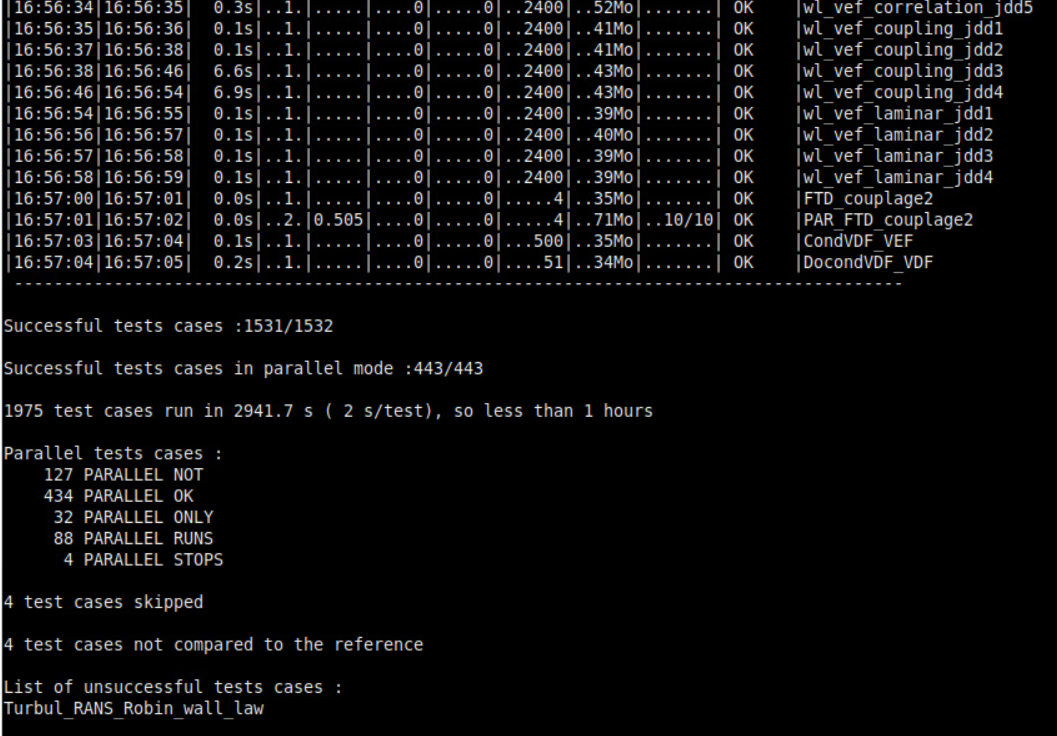
\includegraphics[width=16cm]{pictures/verif-resultats.png}
   \vspace*{0.2cm}
   \captionof{figure}{\label{figure:verif-resultats}Exemple de bilan du lancement de la base de vérification lancée en local}
\end{figure}


Pour le lancement automatique quotidien, l'atelier de TrioCFD,
contenant un ensemble de procédures en Bash et en Python,
est exécuté chaque soir par l'atelier de TRUST par une crontab (procédure de lancement automatique et périodique)
sur le script \texttt{lance\_test\_nuit} contenu dans le répertoire \texttt{bin/admin} de TRUST.
Ce script met à jour TrioCFD par rapport à ce qui a été intégré la veille dans la branche \texttt{triou/TMA},
installe TRUST, puis envoi TriocCFD (et les autres baltiks sur base TRUST) sur les machines du parc (voir tableau \ref{tab:Computer-characteristics}).
Les machines sur lesquelles TRUST et ses Baltiks sont testés chaque nuit sont spécifiées dans le fichier \texttt{bin/admin/liste.machines} de TRUST.
Les machines concernant TrioCFD sont celles qui contiennent le paramètre -TrioCFD
dans ce fichier au niveau de la colonne \texttt{baltiks}.
Ce fichier contient également les options de compilation
et de lancement des tests. Quelques-unes de ces options sont données dans le tableau \ref{tab:options-verif}.

\begin{table}[H]
\begin{centering}
\footnotesize
\begin{tabular}{Sc Sc}
\hline\hline
\rowcolor{lightgray}\textbf{Option} & \textbf{Signification}  \tabularnewline
\hline
-g & lancement des cas tests en mode debug \tabularnewline \hline
-semi\_opt & lancement des cas tests en mode semi optimisé \tabularnewline \hline
-gui & test des balises XDATA (génération Référence Manual) \tabularnewline \hline
-clang & permet de spécifier un compilateur CLANG (variante de compilateur - par défaut GNU) \tabularnewline \hline
-cuda & lancement des tests sur les GPC - par défaut sur les CPU \tabularnewline \hline
-gcov & test la couverture des mots clés par la base de vérification \tabularnewline \hline
-limited & lance une base plus succincte de cas tests (20)\tabularnewline \hline 
-all & lance l'ensemble des cas tests)\tabularnewline \hline
-build\_64\_bit & lancement sur 64 bits \tabularnewline \hline 
-test & lancement des cas tests de TRUST avec l'exécutable de TrioCFD \tabularnewline \hline
-platform & profiling : analyse les temps de passage dans les différentes parties du code \tabularnewline \hline
-disable-mpi & désactive le lancement en parallèle des cas tests \tabularnewline \hline
-download-visit & télécharge la dernière version de Visit plutôt que d'utiliser la version présente dans TRUST  \tabularnewline 
\hline\hline
\end{tabular}
\normalsize
\par\end{centering}
\caption{\label{tab:options-verif}Liste des options utilisées par l'atelier logiciel pour le lancement de la base de vérification}
\end{table}

Le script \texttt{lance\_test\_nuit} installe d'abord TrioCFD sur la machine de l'atelier, puis crée un fichier qui permet de spécifier les options de compilation et de tests pour chacune des machines distantes. Ce fichier s'appelle Run.liste et contient autant de lignes de machines et spécifie, entre autre, le nom de la machine, le chemin vers TRUST, le chemin d'installation, le mode de tests,..\\
Le lancement des installations sur les machines distantes se fait avec le script \texttt{/export/home/\-triou/tuleap/Livraison/TRUST/bin/baltik/share/baltik/bin/baltik\_check\_portability Run.liste}. Ce script va :
\begin{enumerate}
\item créer l'archive triocfd.tar, qui contient le triocfd.tar.gz et les autres scripts pour préparer, installer, configurer, vérifier, ..
\item la copier sur chacune des machines distantes et lancer la compilation
\item récupérer les logs en local de chacune des machines et générer la page nuit\_triocfd.html qui permettra l'analyse des résultats de vérification.
\end{enumerate}


Le script \texttt{lance\_test\_nuit} rapatrie les résultats de TRUST à 7h du matin, et stoppe la procédure de vérification de TrioCFD sur les machines pour lesquelles l'installation ou les tests ne sont pas terminés. Ceci garantit que la page nuit\_triocfd.html est correctement générée. Cette page servira au dépouillement des résultats de la base de vérification.


\subsection{Dépouillement des résultats de la base de cas-tests de \texttt{TrioCFD}}

L'analyse des résultats obtenus par la base de vérification de TrioCFD commence par l'analyse de la page html générée par le script \texttt{lance\_test\_nuit} (voir figure \ref{figure:trio_verif}). Cette page de rapport a été refondue en 2021 afin de faire figurer les éléments nécessaires pour analyser efficacement les résultats de la base de vérification.\smallskip\\
 Elle est composée de 15 colonnes, les colonnes 1, 4, 5 et 6 donnent les informations générales sur les machines testées (nom, OS, architecture, et compilateur C++). Les colonnes 2 et 3 renseignent sur la date et l'heure de démarrage de l'atelier de vérification sur chacune des machines. La $7^{ème}$ colonne identifie si la machine est considérée comme une machine cible (machine sur laquelle le succès de la vérification est indispensable pour considérer la version du jour comme stable). Ces machines sont au nombre de 4 sur TrioCFD. Elles correspondent à des machines présentant une configuration standard en terme d'OS et compilateur par rapport aux machines des utilisateurs/développeurs. Ainsi, si l'atelier de vérification ne fonctionne pas sur ces machines cibles, l'utilisation du code sera dégradée dans l'équipe. La $13^{ème}$ colonne correspond au mode de compilation de de TrioCFD sur la machine concernée. Toutes les autres colonnes sont quant à elles destinées à l'analyse de la base de vérification :\\
\begin{itemize}[label=$\Rightarrow$, font=\LARGE]
   \item \textbf{Colonne 8 - prepare} : vérifie que le désarchivage de l'archive envoyée par la machine de l'atelier s'est bien déroulé et génère les scripts de lancement propres à chaque machine (configure.sh, make.sh,...) en fonction des options définies dans le fichier \texttt{liste.machines}
   \item \textbf{Colonne 9 - configure} : vérifie que la configuration de TrioCFD s'est bien déroulée (commandes \texttt{baltik\_build\_configure et \texttt{./configure}}
   \item \textbf{Colonne 10 - make} : vérifie que la compilation de TrioCFD a été faite avec succès en respectant les options de compilations spécifiées
   \item \textbf{Colonne 11 - make\_check} : lancement des tests de vérification en respectant les options spécifiées dans le fichier \texttt{liste.machines}
   \item \textbf{Colonne 12 - make\_install} : vérifie que l'installation générale a été bien faite et le baltik bien chargé. Cet état est toujours valide si les 4 présents ont abouti avec succès. Cette colonne pourra être supprimée lors de la prochaine évolution de l'atelier de vérification
   \item \textbf{Colonne 14 - test\_par} : nombre de tests en mode parallèle réussis par rapport au nombre de tests lancés
   \item \textbf{Colonne 15 - test\_seq} : nombre de tests en mode séquentiel réussis par rapport au nombre de tests lancés
\end{itemize}

Le résultat pour chacune de ces 6 colonnes est analysable dans le détail en cliquant sur le lien présent dans chacune des cases qui renvoie aux fichiers \texttt{.log} ou \texttt{.err}. L'équipe TMA assure le suivi quotidien du bon déroulement de l'atelier de vérification. En cas de problème, l'équipe TMA et les Responsable de Code s'attacheront à résoudre au plus vite les problèmes constatés et aucune nouvelle intégration ne sera faite dans la branche en développement de TrioCFD tant que l'état de l'atelier de vérification ne sera pas revenu dans son état nominal. 
\newpage

\begin{figure}[H]
   \centering
   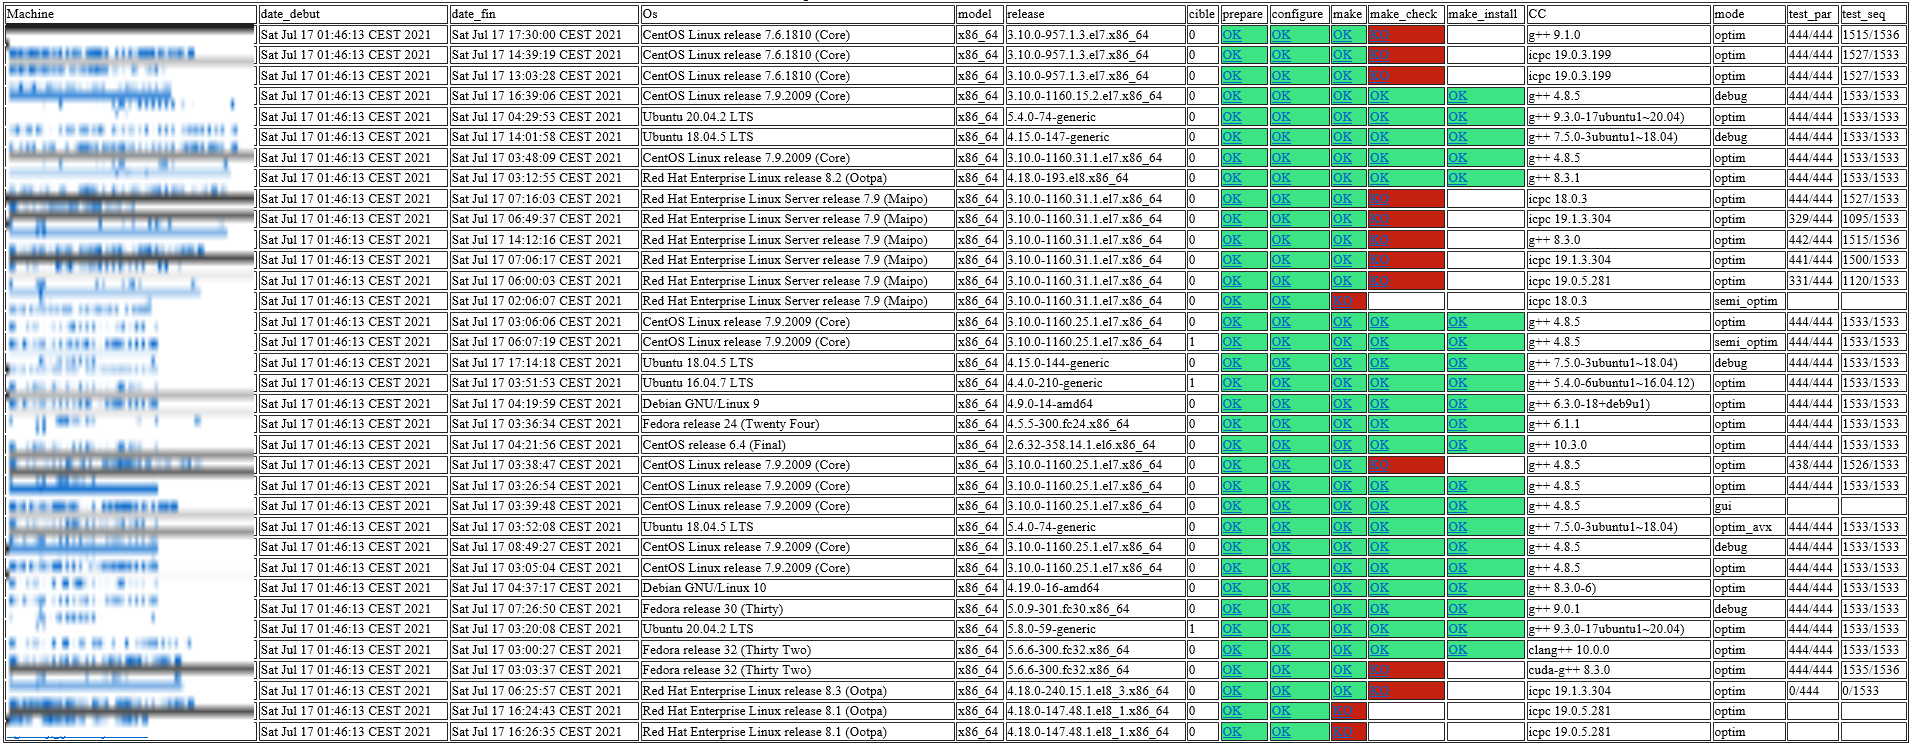
\includegraphics[width=23cm ,angle =90]{pictures/trio_verif_flou.png}
   \vspace*{0.2cm}
   \captionof{figure}{\label{figure:trio_verif}Page html générée pour l'analyse quotidienne de la base de vérification de TrioCFD}
\end{figure}




%%%%%%%%%%%%%%%%%%%%%%%%%%%%%%%%%%%%%%%%%%%%%%%%%%%%%%%%%%%%%%%%%%%%%%%%%%%%%%%%%%%%%%%%%%%%%%%%%%%%%%%%%%%%%%%%%%%%%

\chapter{\label{chapitre:validation}Base de Validation de TrioCFD}
\lhead{Base de Validation}
\rhead{DESCRIPTION DES OUTILS DE V\&V}
Si la v\'erification logicielle garantit que le r\'esultat de chaque phase du processus de d\'eveloppement logiciel r\'ealise effectivement les sp\'ecifications initiales (\textit{e.g.} impl\'ementation correcte des \'equations et mod\`eles sp\'ecifi\'es initialement), la validation logicielle garantit, quant \`a elle, que le produit logiciel r\'epond aux besoins de toutes les parties prenantes (\textit{e.g.} la bonne r\'esolution des \'equations d\'efinies dans les sp\'ecifications et r\'esultats physiques conformes \`a l'attendu).

\subsection{La base de validation de \texttt{TrioCFD}}

La validation du code est effectuée via les fiches/rapports de validation.
Ces rapports peuvent être composées d'un ou plusieurs cas tests de la base de vérification.
Lorsqu'une fiche de validation est composée de plusieurs cas tests, c'est parce que ceux-ci comportent des variantes (différents maillages, différents modèles,...).
Le nombre de rapports de la base de validation augmente r\'eguli\`erement.
En effet, \`a chaque nouveau d\'eveloppement, un nouveau rapport de validation doit \^etre ajout\'e pour de le tester.\\
Les rapports de validation sont disponibles dans le répertoire \texttt{/share/Validation/Rapports\_automatiques}.
Ils peuvent être ensuite ordonnées dans différents sous-répertoires pour mieux identifier les sujets d'intérêt de chacun.\\

Le tableau récapitulatif des différentes fiches de validation est donné en Annexe A du document intitulé "TrioCFD\_models\_report.pdf" présent dans le répertoire \texttt{share/doc} de TrioCFD.
Il sera amené à être prochainement migré vers le document validation\_report\_TrioCFD.pdf situé dans ce même répertoire.\\

La validation de r\'ef\'erence est actuellement exécutée sur la machine \emph{uruk} (Ubuntu20, gcc 9.4.0).\\
Les autres clusters (voir \ref{tab:Computer-characteristics}) sont des machines partagées avec d'autres codes,
le processus de validation nécessite trop de temps de calcul et les stations ne sont pas suffisamment puissantes
pour que le processus de validation soit achevé dans des temps raisonnables.\\

Le processus de validation présente également une contrainte forte en terme de temps de résolution
et doit être en mesure de fournir les résultats dans un délai acceptable (quelques jours au plus).\\

La base de validation est exécutée via le logiciel Open Source \emph{Jenkins},
qui permet de bien gérer tous les processus d'un code en intégration continue comme TrioCFD.
Jenkins fournit une interface graphique simple pour la création de files de tâches ainsi qu'un mode un peu plus évolué
avec la possibilité pour l'utilisateur d'implémenter ses propres scripts en langage Groovy.\\
TrioCFD utilise ces deux fonctionnalités de Jenkins pour le lancement de la base de validation de TrioCFD.\\
La validation hebdomadaire du logiciel porte actuellement sur les aspects suivants :
\begin{itemize}[label=$\Rightarrow$, font=\LARGE]
   \item \textbf{la bonne compilation du code}
   \item \textbf{la bonne résolution des fiches de validation}
   \item \textbf{la bonne génération des fiches de validation}
\end{itemize}

Ce processus de validation sera prochainement enrichi afin d'être également en mesure de contrôler la portabilité du code de façon plus poussée que la base de vérification mais s'assure également de la bonne génération de la documentation utilisateur de TrioCFD.\\

\subsection{Fréquence de lancement de la base de validation de \texttt{TrioCFD}}
La base de validation est ex\'ecut\'ee de façon hebdomadaire.
Son lancement est actuellement réalisé manuellement par le Responsable de Code le vendredi,
après que les dernières intégrations prévues dans la branche \texttt{triou/TMA} aient été réalisées.
Ce lancement hebdomadaire est réalisé sur la branche en développement de TrioCFD en s'appuyant sur la version de même niveau de TRUST.\\
Lorsque des développements pour lesquels des impacts sont prévus doivent être intégrés dans la version,
la base de validation peut être amenée à être lancée àtout moment par le Responsable de Code.

\subsection{Méthodologie de lancement de la base de validation de \texttt{TrioCFD}}

La machine maître de lancement des tâches de Jenkins (Pipelines) est actuellement la station 9 du tableau \ref{tab:Computer-characteristics}.
Un Pipeline spécifique a été créé pour le lancement de la validation, nommé TrioCFD\_Validation et rattaché au cluster 2.
Ce Pipeline est lancé manuellement en remplissant la fiche de paramètres de la figure \ref{figure:lancement_jenkins}.

\begin{figure}[H]
   \centering
   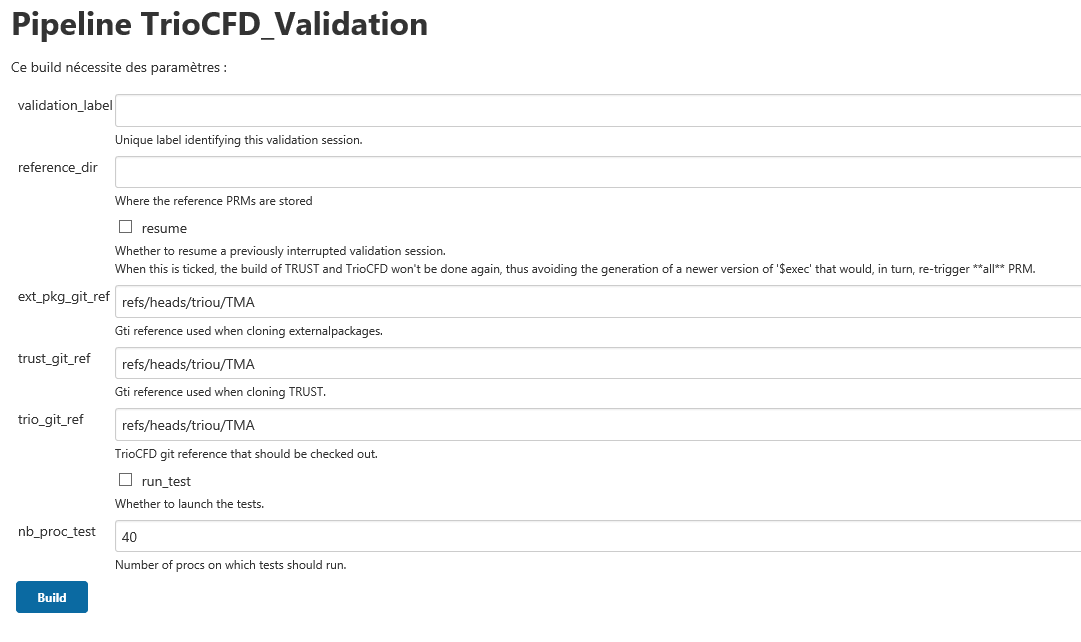
\includegraphics[width=16cm]{pictures/lancement_jenkins.png}
   \vspace*{0.2cm}
   \captionof{figure}{\label{figure:lancement_jenkins}Méthodologie de lancement du Pipeline de Validation de TrioCFD sous Jenkins}
\end{figure}
Six principaux paramètres sont à renseigner manuellement pour le lancement de la base de validation qui sont :
\begin{itemize}[label=$\Rightarrow$, font=\LARGE]
   \item \textbf{validation\_label} : nom du répertoire de validation résultant de ce lancement
   \item \textbf{reference\_dir} : nom du répertoire d'une version antérieure de validation par rapport à laquelle la version lancée sera comparée
   \item \textbf{ext\_pkg\_git\_ref} : branche, SHA1 ID ou tag du dépôt git de externalpackages à partir duquel la validation sera lancée
   \item \textbf{trust\_git\_ref} : branche, SHA1 ID ou tag du dépôt git de TRUST à partir duquel la validation sera lancée
   \item \textbf{trio\_git\_ref} : branche, SHA1 ID ou tag du dépôt git de TrioCFD à partir duquel la validation sera lancée
   \item \textbf{nb\_proc\_test} : nombre de processeurs de la machine sur laquelle le processus de validation sera lancé (par défaut 40)
\end{itemize}
Deux cases à cocher sont utilisées pour la réitération du lancement en cas de problème lors du précédent.
La première, nommée \texttt{resume} permet de relancer le processus de validation à partir de l'endroit exact où celle-ci a été interrompu.
La seconde, nommée \texttt{run\_test}, permet de s'affranchir de toute la première partie qui concerne le clonage des différentes bases git de la compilation de TRUST et TrioCFD.

Ce Pipeline lance le script \texttt{TrioCFD\_validation.gy} présent dans le répertoire \texttt{/home/service/s-sac-dm2s-trust-tri/jenkins/scripts/} avec en arguments,
les paramètres précédemment renseignés.
Ce script Groovy est composé de plusieurs étapes :
\begin{enumerate}
\item \textbf{check-ref-dir} : vérification de l'existence du répertoire de la version de référence (2ème paramètre de la figure ci-dessus)
\item \textbf{git-ext-pkg} : clonage du dépôt GIT externalpackages et positionnement par rapport au paramètre renseigné dans \texttt{ext\_pkg\_git\_ref}
\item \textbf{git-TRUST} : clonage du dépôt GIT TRUST et positionnement par rapport au paramètre renseigné dans \texttt{trust\_git\_ref}
\item \textbf{configure-TRUST} : configuration de TRUST
\item \textbf{build-optim-TRUST} : compilation de TRUST en mode optimisé
\item \textbf{configure-MEDICoCo} : configuration des outils de couplage (MEDCoupling et ICoCo)
\item \textbf{build-optim-MEDICoCo} : compilation des outils de couplage en mode optimisé
\item \textbf{git-TrioCFD} : clonage du dépôt GIT TRUST et positionnement par rapport au paramètre renseigné dans \texttt{trio\_git\_ref}
\item \textbf{configure-TrioCFD} : construction et configuration de TrioCFD
\item \textbf{build-optim-TrioCFD} : compilation de TrioCFD en mode optimisé
\item \textbf{prepare\_valid} : génération du makefile de la validation et des fichiers CTest (fiches de validation à lancer)
\item \textbf{clean\_status} : nettoyage des résultats du précédent lancement
\item \textbf{ctest\_valid} : lancement des fiches de Validation, génération du répertoire des résultats de ce lancement suivant le paramètre renseigné dans \texttt{validation\_label}, création de la page html de résultat et bilan sur l'état de chaque fiche de validation dès qu'une arrive à son terme
\item \textbf{ctest\_valid\_agg} : finalisation du processus de validation
\end{enumerate}

Le suivi de l'avancée du processus de validation se fait en direct dans Jenkins et permet de savoir,
à tout moment, où en est le processus mais également connaître le bon déroulé ou non
de chaque étape et le temps pris par chacun (voir figure \ref{figure:etapes_validation}).

\begin{figure}[H]
   \centering
   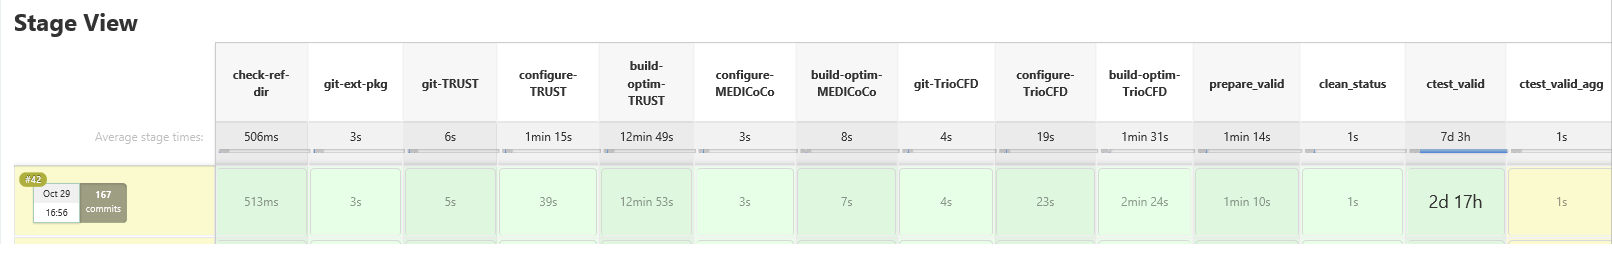
\includegraphics[width=16cm]{pictures/etapes_validation.png}
   \vspace*{0.2cm}
   \captionof{figure}{\label{figure:etapes_validation}Les différentes étapes du processus de Validation de TrioCFD sous Jenkins}
\end{figure}

Une fois le processus arrivé dans l'étape \texttt{ctest\_valid},
l'état de chaque fiche peut être consulté en temps réel dans la page html de suivi qui sera décrite dans la section suivante.\\

Durant la validation, les résultats sont stockés
dans le répertoire \texttt{/volatile/projet/trust\_trio/jenkins/workspace/TrioCFD\_Validation\_\{nomDeLaMachine\}/validation}.\\

A la fin du processus de validation, ce r\'epertoire de calcul est copi\'e
dans le r\'epertoire \texttt{/volatile/projets/trust\_trio/validation/TrioCFD} de la machine de validation.\\
Ce r\'epertoire comprendra donc l'ensemble des r\'esultats de validation obtenus
entre les versions officielles \emph{n} et \emph{n+1} de TrioCFD.\\

Enfin, lors de la mise en service d'une version majeure,
le r\'epertoire de calcul est archiv\'e dans le r\'epertoire  \texttt{/home/trust\_trio/validation}.


\subsection{Dépouillement des résultats de la base de validation de \texttt{TrioCFD}}

Pour le dépouillement des résultats, le script Groovy \texttt{TrioCFD\_validation.gy}
génère une page HTML consultable depuis l'interface Jenkins, ou pouvant être ouverte
par le biais d'un navigateur web.
Il s'agit du fichier \texttt{prm\_report.html} qui se trouve dans le r\'peroire de calcul.
Cette page est composée de cinq rubriques.\smallskip\\

\begin{minipage}[c]{0.65\linewidth}
La première nommée \textbf{Summary} est un résumé du nombre de fiches ayant tourné avec succès et des fiches en échec.
Par échec, on entend à la fois les fiches n'ayant pas abouti et les fiches présentant des écarts avec la version de référence.
\end{minipage} \hfill
\begin{minipage}[c]{0.3\linewidth}
   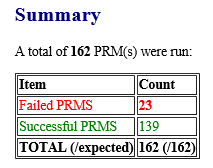
\includegraphics[width=5cm]{pictures/validation-summary.png}\vspace*{0.2cm}
   \captionof{figure}{Dépouillement résultats de validation - partie 1 : Summary}
\end{minipage}
\vspace{0.5cm}

La deuxième nommée \textbf{Running PRMS} liste les fiches de validation en cours de calcul lorsque la page HTML est consultée avant la fin du processus de validation.\vspace{0.6cm}\\


\begin{minipage}[c]{0.5\linewidth}
La rubrique 3, \textbf{Failed PRMS (run failed)}, correspond à un tableau des fiches de validation qui ont planté. Le plantage peut être dû à l'échec d'un des jdds de la fin de validation ou à une erreur lors de la génération du pdf de la fiche.
\end{minipage} \hfill
\begin{minipage}[c]{0.45\linewidth}
   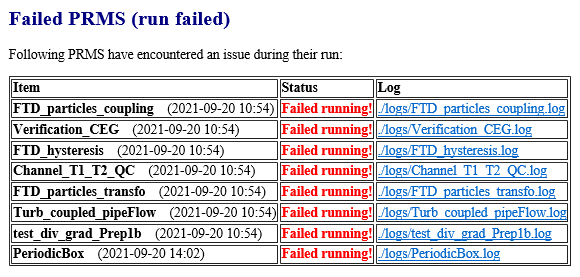
\includegraphics[width=8cm]{pictures/validation-PRMSfailed.png}\vspace*{0.2cm}
   \captionof{figure}{Dépouillement résultats de validation - partie 3 : Failed PRMS}
\vspace{0.6cm}   
\end{minipage}
\vspace{0.6cm}

La quatrième nommée \textbf{Failed PRMS (comparison)} correspond aux fiches ayant tourné avec succès, mais qui présentent des écarts par rapport à la version de référence. Ces écarts sont détectés automatiquement par une comparaison pixel à pixel du nouveau pdf généré et du pdf de la version de référence. C'est alors au Responsable de Code d'intervenir pour faire une analyse manuelle de ces écarts. Ceux-ci peuvent être sans réelle importance et correspondre seulement à un décalage d'une ligne sur le pdf nouvellement généré par rapport à la fois précédente, ou à une légère variation du temps de calcul. A contrario, cet échec de comparaison peut venir d'un impact physique ou numérique important qui devra être justifié ou corrigé.\vspace{0.9cm}   \\

\begin{minipage}[c]{0.25\linewidth}
   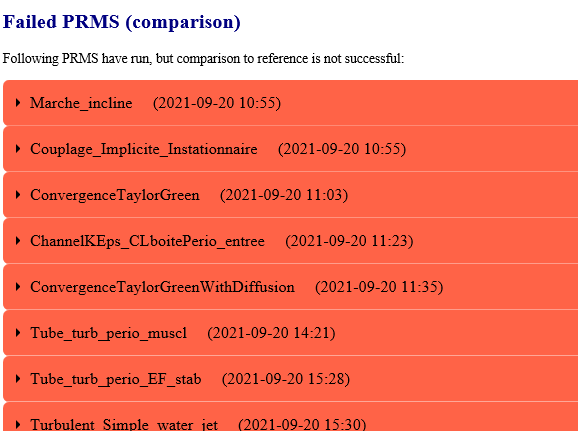
\includegraphics[width=4cm]{pictures/validation-PRMSfailedcomp.png}\vspace*{0.2cm}
   \captionof{figure}{Dépouillement résultats de validation - partie 4 : Failed PRMS au niveau de la comparaison des PDF}
\end{minipage} \hfill
\begin{minipage}[c]{0.7\linewidth}
   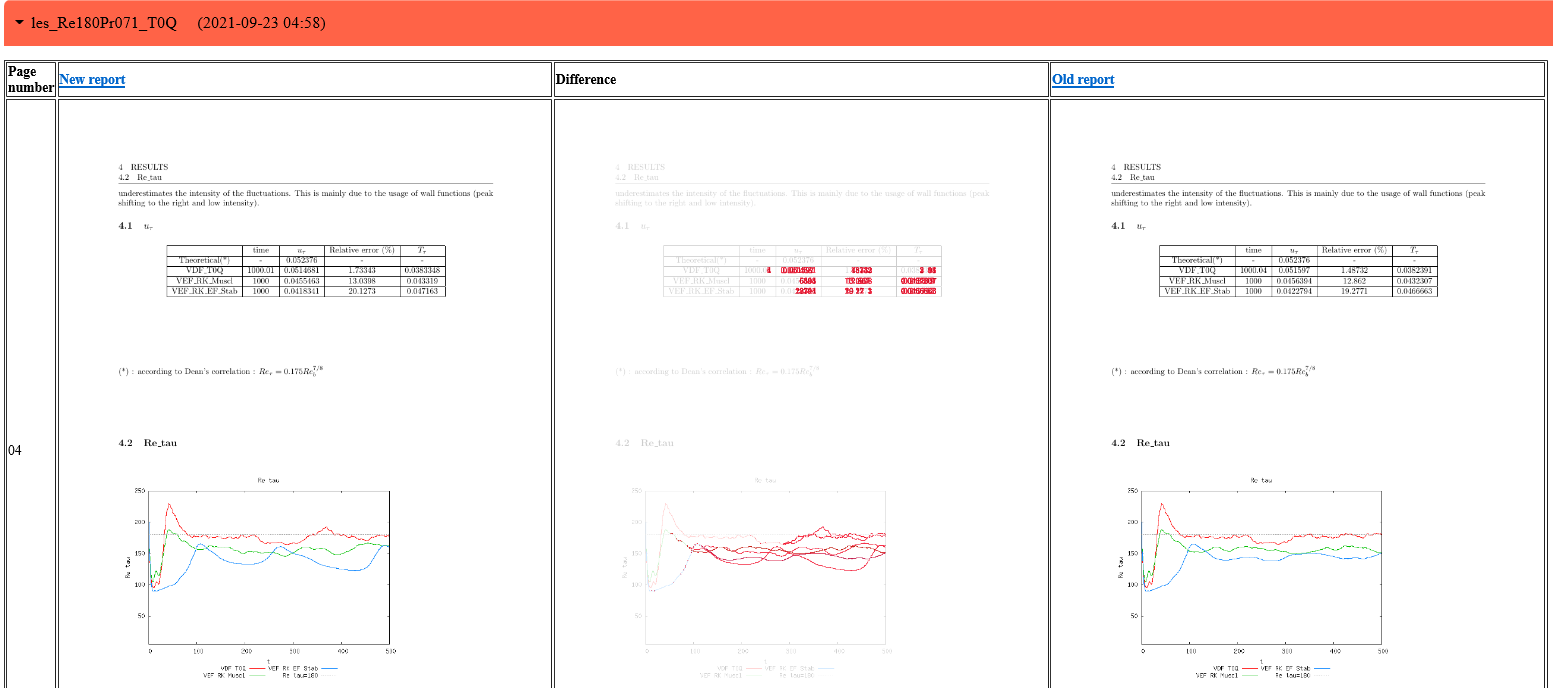
\includegraphics[width=12cm]{pictures/validation-comparepdf2.png}\vspace*{0.2cm}
   \captionof{figure}{Dépouillement résultats de validation - partie 4 : Failed PRMS, exemple de comparaison pixel à pixel}
\end{minipage}
\vspace{0.5cm}

\begin{minipage}[c]{0.5\linewidth}
La dernière partie (\textbf{Successful PRMS} récapitule l'ensemble des fiches de validation
qui ont été générées correctement et qui ne présentent aucun écart par rapport à la version de référence.
\end{minipage} \hfill
\begin{minipage}[c]{0.45\linewidth}
   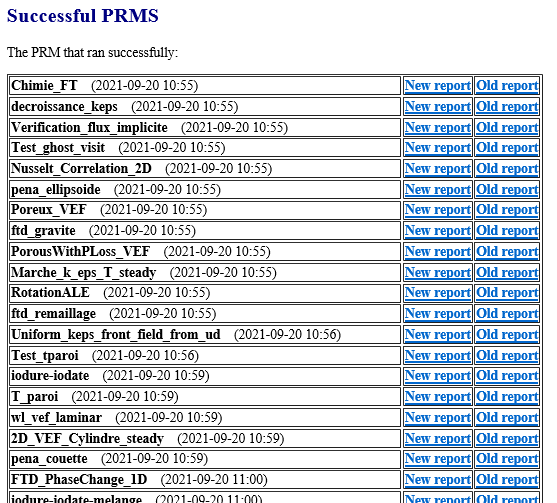
\includegraphics[width=8cm]{pictures/validation-success.png}\vspace*{0.2cm}
   \captionof{figure}{Dépouillement résultats de validation - partie 5 : Successfull PRMS}
\vspace{0.6cm}   
\end{minipage}

